\begin{itemize}
    \item Radiation Survey Monitor
    \item Pocket Dosimeter
\end{itemize}

\textbf{Radiation Survey Monitor:} A radiation survey monitor is a portable device used to measure and detect ionizing radiation levels in various environments. It typically consists of a Geiger-Müller tube or scintillation detector that can detect different types of radiation, such as alpha, beta, gamma, and X-rays. The monitor provides real-time readings of radiation intensity, allowing users to assess potential radiation hazards and ensure safety in areas where radioactive materials are present.

\begin{enumerate}
    \item \textbf{Pressurized Ionization Chamber Survey Meter:} This type of survey meter uses a pressurized ionization chamber to detect and measure ionizing radiation. It is particularly effective for measuring high levels of gamma and X-ray radiation. The pressurized chamber increases the sensitivity of the device, allowing for accurate readings even in low radiation environments.
    
    \textbf{Fluke 451P:} The Fluke 451P is a specific model of a pressurized ionization chamber survey meter known for its precision and reliability. It is widely used in medical, industrial, and environmental applications to monitor radiation levels and ensure compliance with safety standards. \textbf{Key features} of the Fluke 451P include:
    \begin{itemize}
        \item High µR sensitivity measurement of rate and dose simultaneously
        \item Records peak rate using “Freeze Mode”
        \item Auto-ranging and auto-zeroing
        \item Ergonomic, anti-fatigue handle with replaceable grip, wrist strap and tripod mount
        \item Available with dose equivalent energy response (SI units)
        \item Programmable flashing LCD display
    \end{itemize}
    \item \textbf{Geiger-Müller (GM) Survey Meter:} The GM survey meter utilizes a Geiger-Müller tube to detect ionizing radiation. It is widely used for its ability to detect a wide range of radiation types, including alpha, beta, and gamma radiation. The GM survey meter provides audible and visual indications of radiation levels, making it easy to use in various settings.
    
    \textbf{Nucleonix RM701N:} The Nucleonix RM701N is a specific model of a Geiger-Müller survey meter known for its versatility and ease of use. It is commonly employed in radiation safety, environmental monitoring, and emergency response situations. \textbf{Key features} of the Nucleonix RM701N include:
    \begin{itemize}
        \item Microcontroller based design.
        \item Compact, elegant and light weight
        \item Uses energy compensated GM Counter.
        \item Accuracy+/- 15\% with Cs-137.
        \item Measures Dose in mR/hr or µSv/hr.
        \item Works on 6V (1.5X4V) dry cell batteries.
        \item IP rating is better than IP56.
        \item Response Time: $<$ 5 seconds.
    \end{itemize}
\end{enumerate}



\textbf{Pocket Dosimeter:} A pocket dosimeter is a small, portable device used to measure an individual's exposure to ionizing radiation over a period of time. It is typically worn on the person, such as on a lapel or pocket, and provides a direct reading of the accumulated radiation dose. Pocket dosimeters are commonly used by radiation workers to monitor their exposure and ensure it remains within safe limits.

\textbf{Mini Electronic Pocket Gamma Dosimeter:} The Digital Dosimeter MPD 1501 is a reliable, lightweight, and convenient personal electronic dosimeter designed for the accurate monitoring of individual X and Gamma radiation exposure.
\newpage
\textbf{Features: }
\begin{itemize}
    \item Based on semiconductor diode detector
    \item Upward replacement for quartz fiber ion chamber dosimeter
    \item Convenient PEN-type design
    \item Light weight $<$ 60gm
    \item Excellent immunity to EMI upto 100V/cm, ERTL certified
    \item unaffected by Mobile phones in close proximity
    \item Over 2500 hrs of continuous operation without battery change
\end{itemize}
\begin{figure}[H]
    \centering
    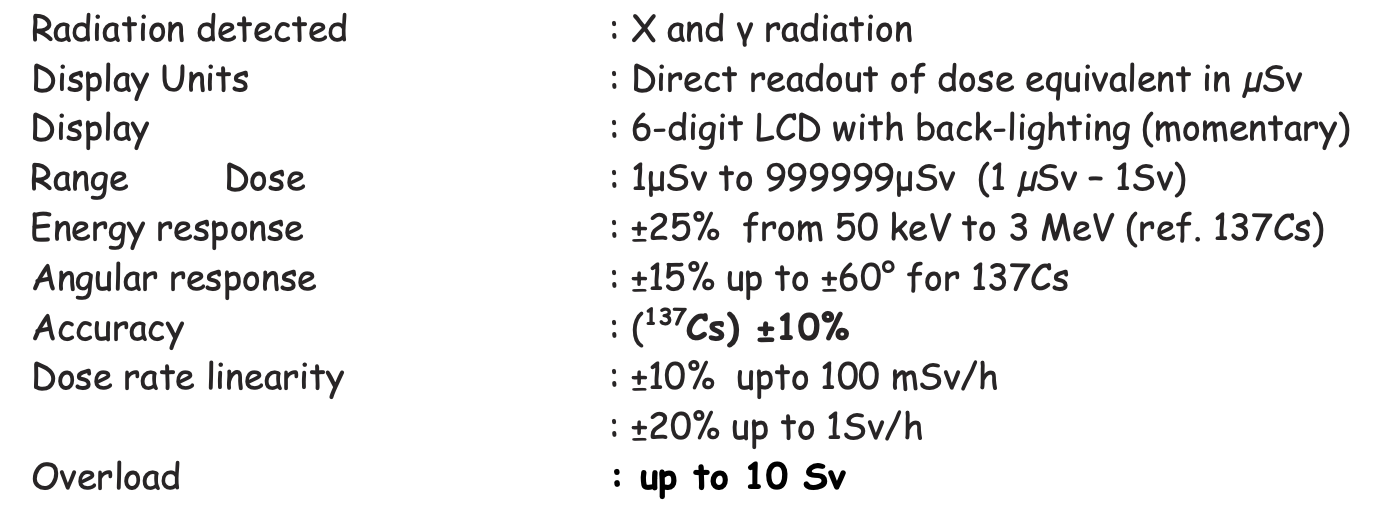
\includegraphics[width=0.7\textwidth]{Figures/Apparatus/Pocket dosimeter spec.png}
\end{figure}

%three figures side by side using sub figure
\begin{figure}[H]
    \centering
    \begin{subfigure}{0.3\textwidth}    
        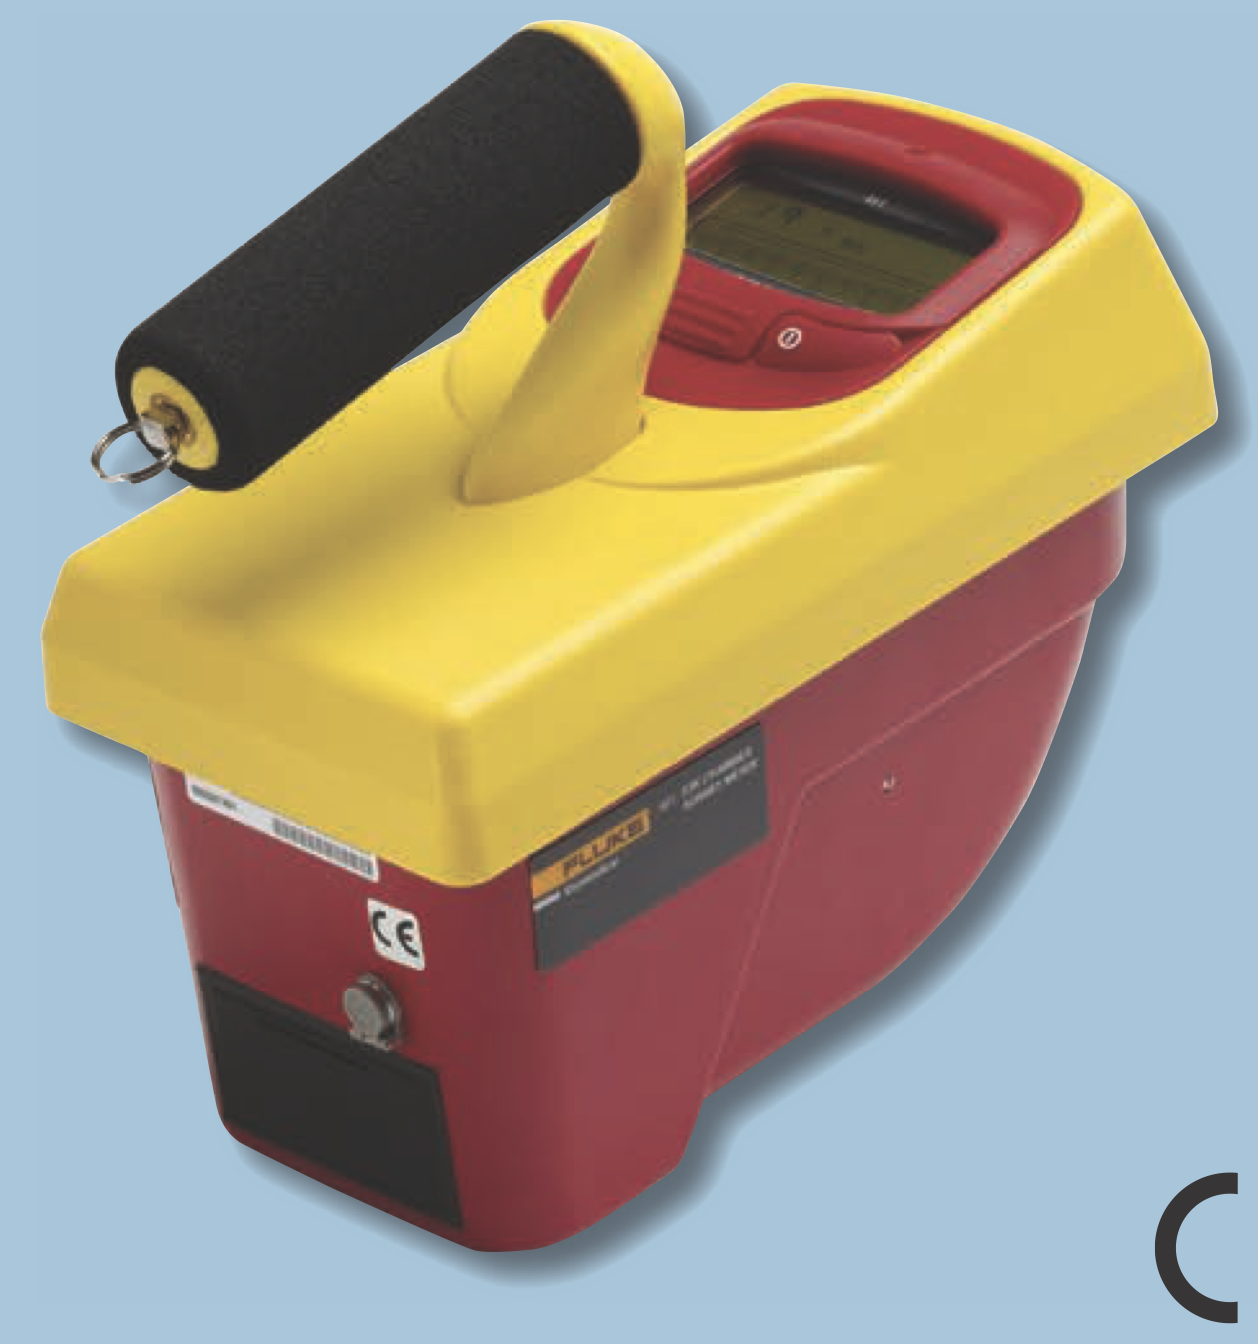
\includegraphics[width=\textwidth]{Figures/Apparatus/Fluke 451P.png}
        \caption{Flukke 451P}
    \end{subfigure}
    \hfill
    \begin{subfigure}{0.3\textwidth}
        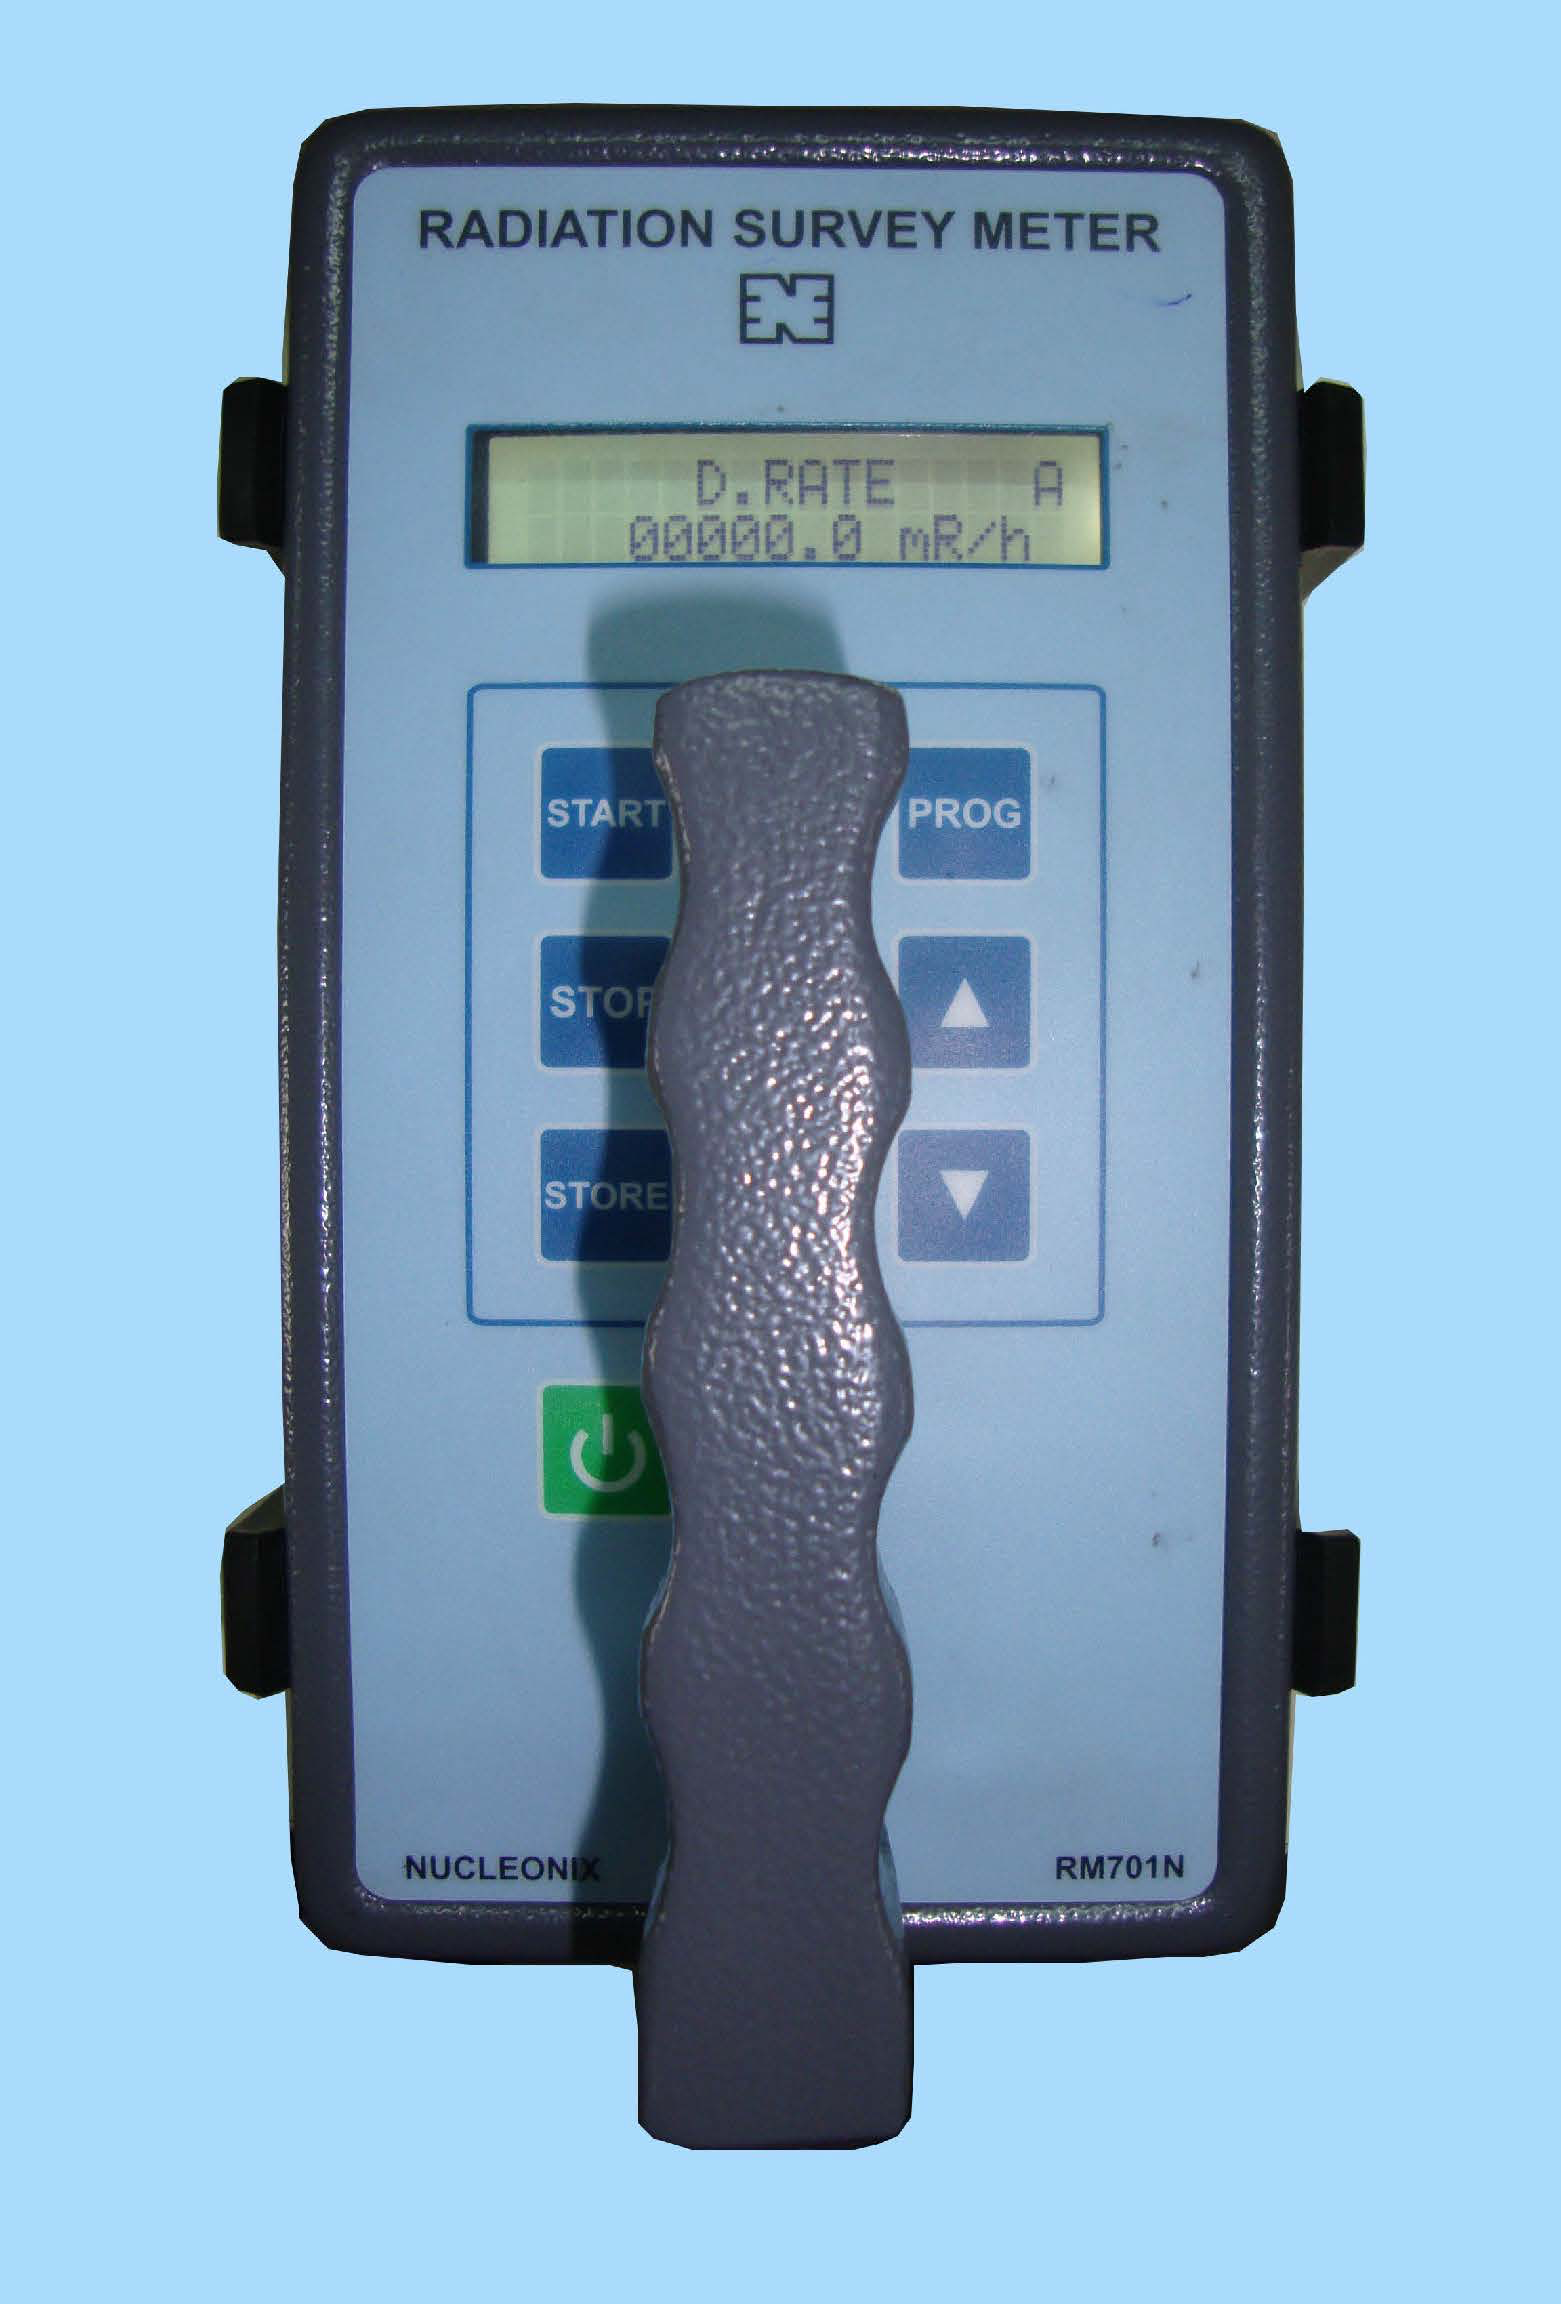
\includegraphics[width=\textwidth]{Figures/Apparatus/Nucleonix.png}
        \caption{Nucleonix RM701N}
    \end{subfigure}
    \hfill
    \begin{subfigure}{0.3\textwidth}
        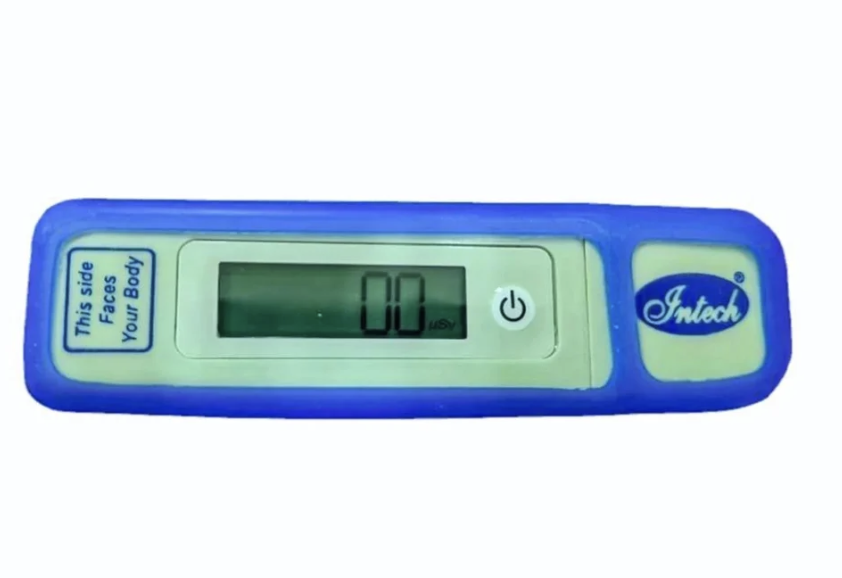
\includegraphics[width=\textwidth]{Figures/Apparatus/PocketDosimeter.png}
        \caption{Pocket Dosimeter MPD 1501}
    \end{subfigure}
    \caption{Various Radiation Survey Instruments}
\end{figure}
